\chapter{序列图建模}
在[协议]下的[顺序图]选项卡中有若干的顺序图面板,在窗体菜单[模型]或快捷按钮中均可添加顺序图。

\section{对象-生命线}
点击小按钮栏目上的[对象-生命线]按钮可以添加一组对象-生命线,如图\ref{obj_lifeline}所示。
\begin{figure}[h]
	\centering
	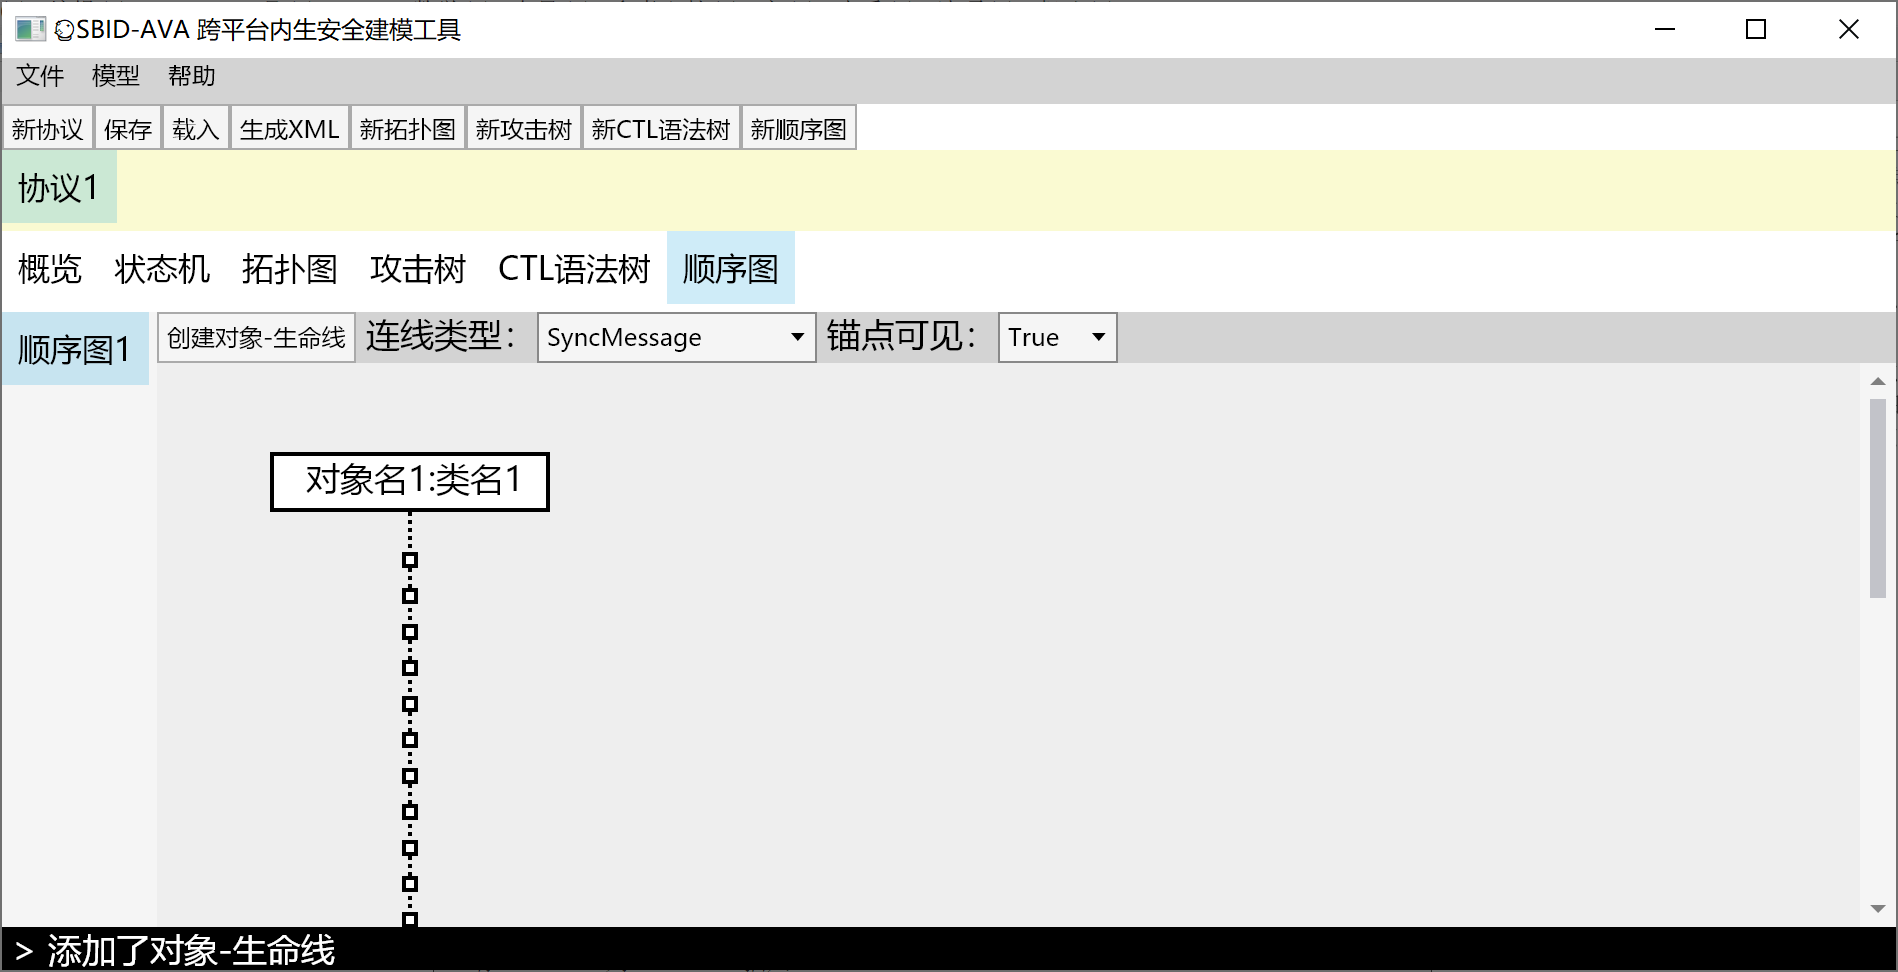
\includegraphics[width=12cm,height=6.75cm]{imgs/obj_lifeline.png}
	\caption{创建对象-生命线}
	\label{obj_lifeline}
\end{figure}
\par
右键对象方框,在右键菜单中选择[编辑对象-生命线],即可打开编辑窗口实时编辑,如图\ref{obj_edit}所示。
\begin{figure}[h]
	\centering
	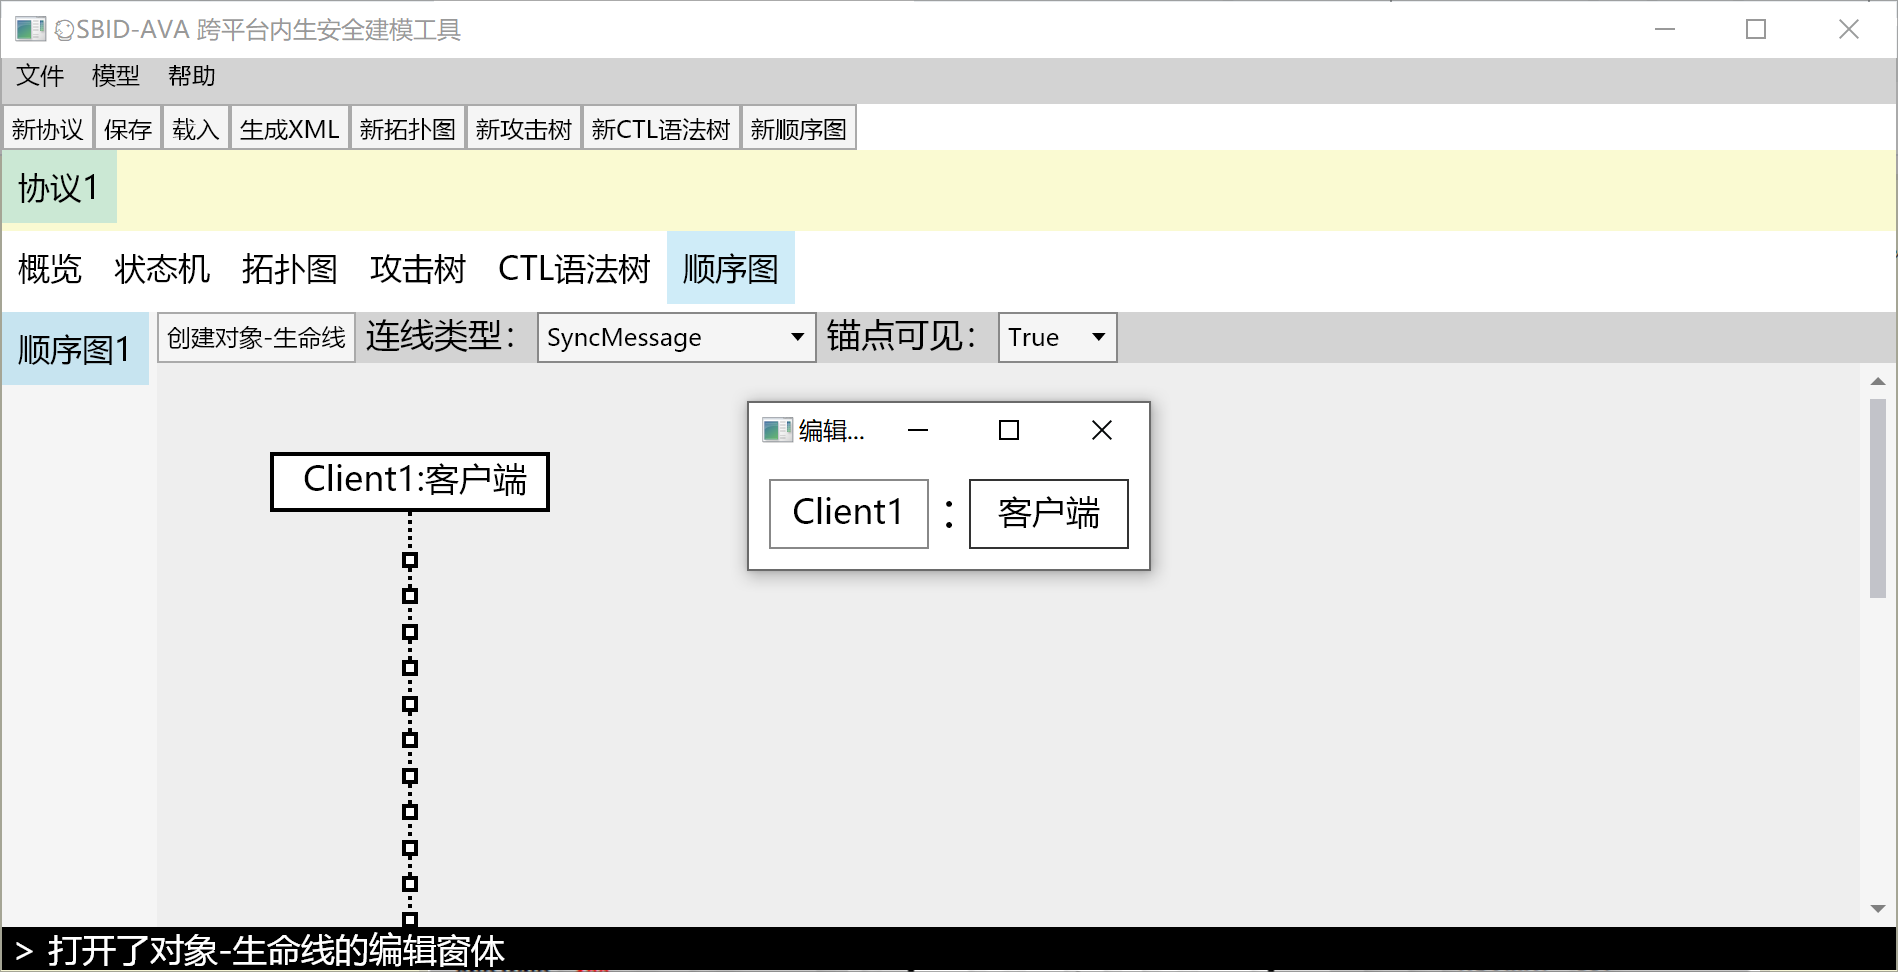
\includegraphics[width=12cm,height=6.75cm]{imgs/obj_edit.png}
	\caption{编辑对象-生命线}
	\label{obj_edit}
\end{figure}

\section{消息传递}
在连线类型中可选三种基本消息,SyncMessage是同步消息,AsyncMessage是异步消息,ReturnMessage是返回消息,点击对象-生命线之间的锚点即可进行消息连线,连线完成后,可以将锚点隐藏,如图\ref{sequencediagram_simple}所示。
\begin{figure}[h]
	\centering
	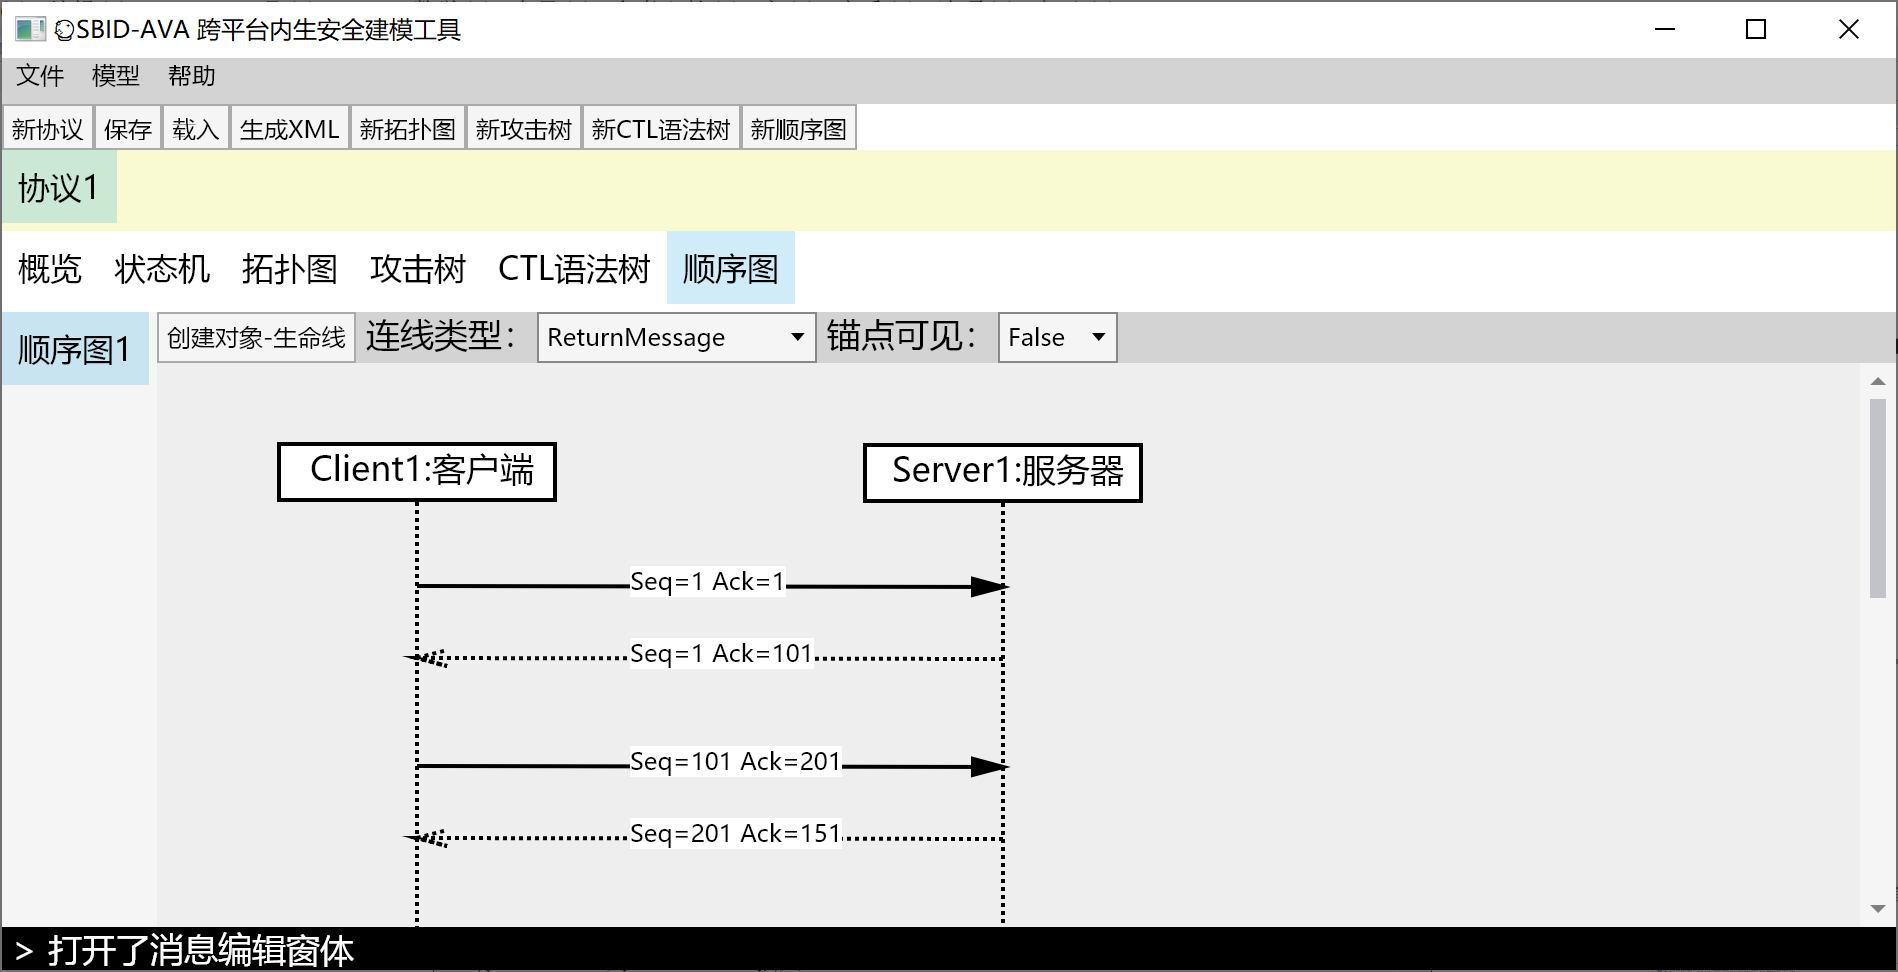
\includegraphics[width=12cm,height=6.75cm]{imgs/sequencediagram_simple.png}
	\caption{简单的连线例子}
	\label{sequencediagram_simple}
\end{figure}
\par
需要注意,SyncMessage和AsyncMessage也可以从自己出发,到自己结束,如图\ref{sequencediagram_simple2}是为服务器添加了到自己的异步消息后的顺序图。
\begin{figure}[h]
	\centering
	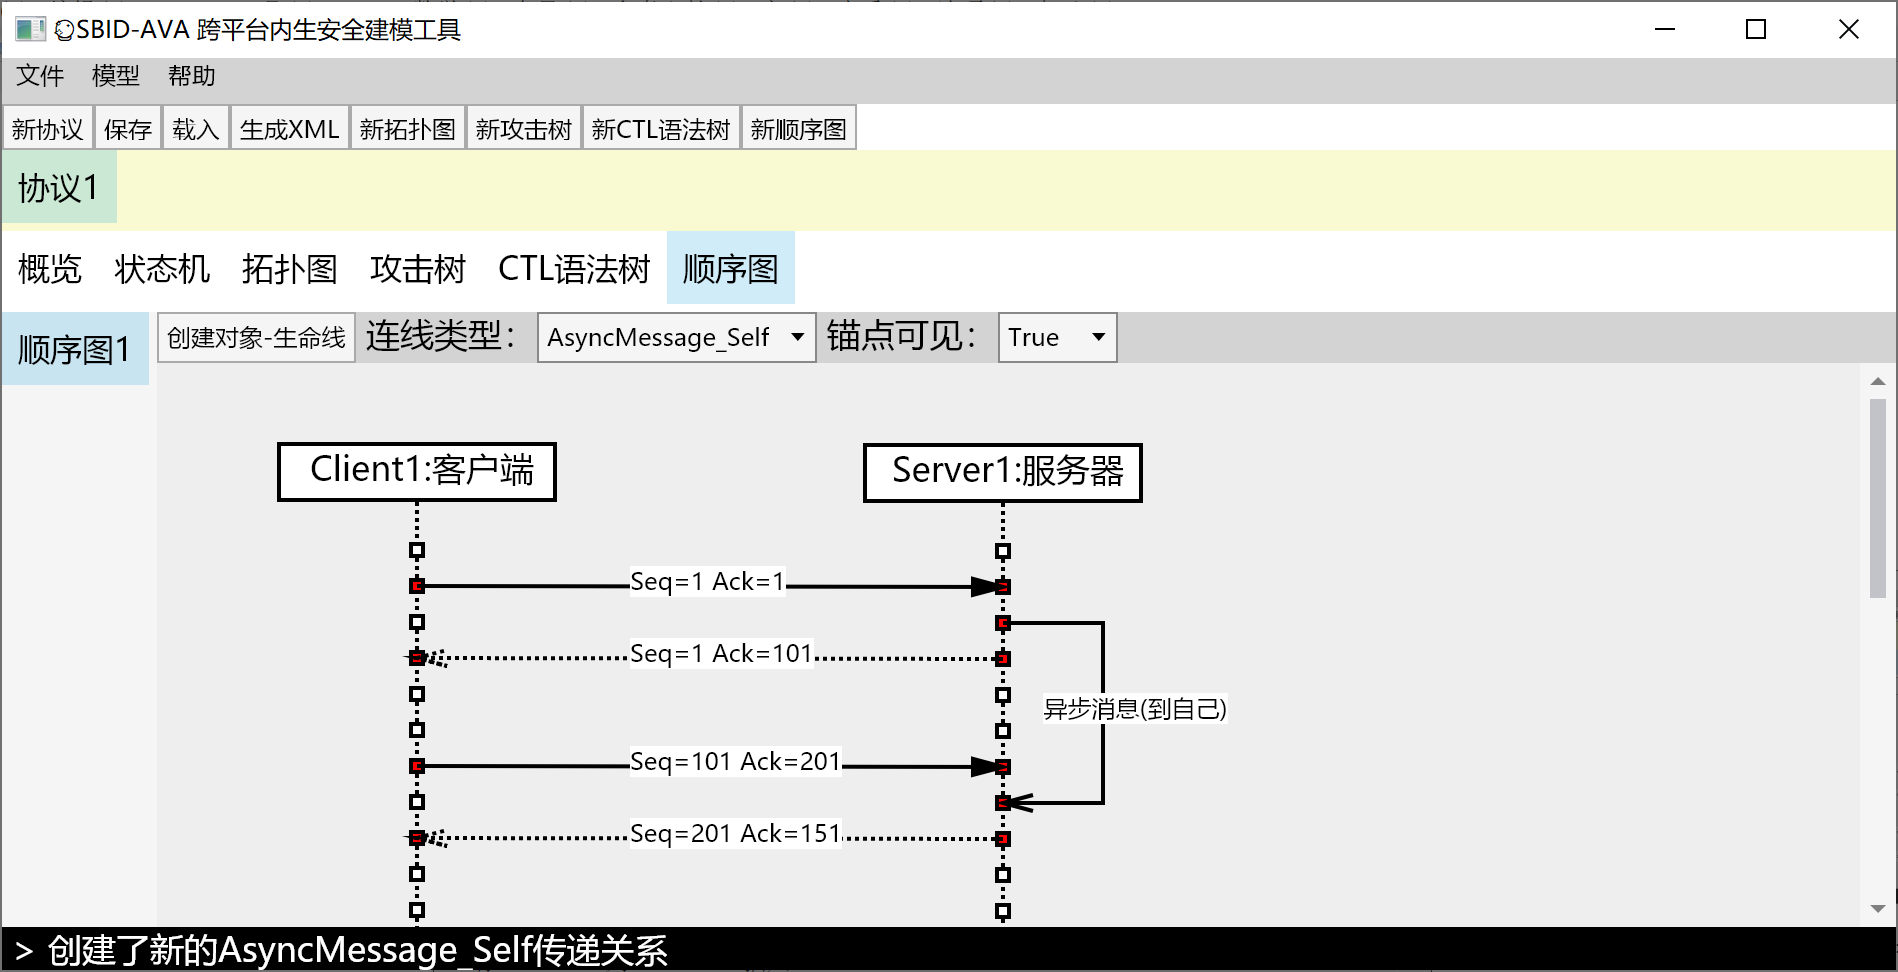
\includegraphics[width=12cm,height=6.75cm]{imgs/sequencediagram_simple2.png}
	\caption{添加到自身的异步消息}
	\label{sequencediagram_simple2}
\end{figure}